\begin{wrapfigure}[20]{r}{0.5\linewidth}
\centering
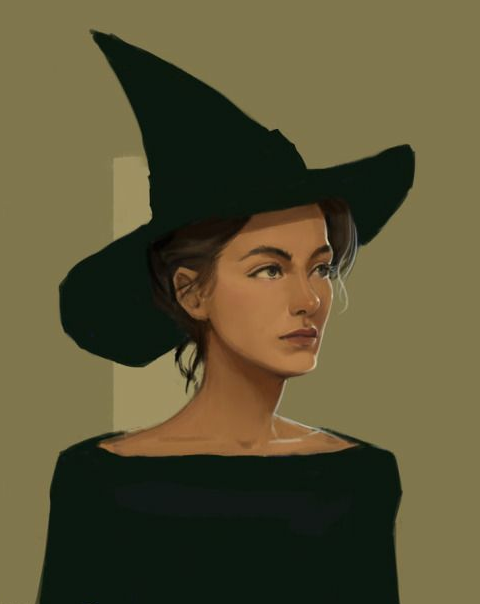
\includegraphics[max width=0.5\textwidth]{../Pictures/Characters/Portraits/Minerva_portrait.png}
\end{wrapfigure}

\paragraph{Description}
Minerva is a black-haired half-blood witch, daughter of his muggle father and her witch mother.

She is a talented student at the Hogwarts School of Witchcraft and Wizardry: after an Hatstall, which took the Sorting Hat five and a half minutes to decide if she was Gryffindor or Ravenclaw, she was Sorted into Gryffindor House. 

Minerva is a Quidditch enthusiast and is particularly gifted at it too: this made her quite popular, letting her make a handful of friends including the shy and overlooked Myrtle Warren of the Ravenclaw House.

She has a soft spot for Transfiguration classes, a quality that made her the most outstanding student in this subject; her professor Dumbledore, charmed by her wits and her resourcefulness, decided to take her under his wing, ready to prepare Minerva for the greatest of the transfiguration skills: the Animagus transformation.

\paragraph{Backstory}
Minerva was born in a complicated family: her father Robert was a muggle Reverend while her mother Isobel was a successful Hogwarts-educated witch. After many years she confessed to her husband, which remained shocked and speechless. The trust between the spouses suffered a heavy hit, however they decided to stay together for the sake of their love and their children.

This event left a scar in Minerva, making her aware of the difficulties of the relationship between muggles and wizards; for this reason, she tried her best to help his two brothers to accept and control their magic abilities while growing in an all-muggle world.

\begin{figure}[H]
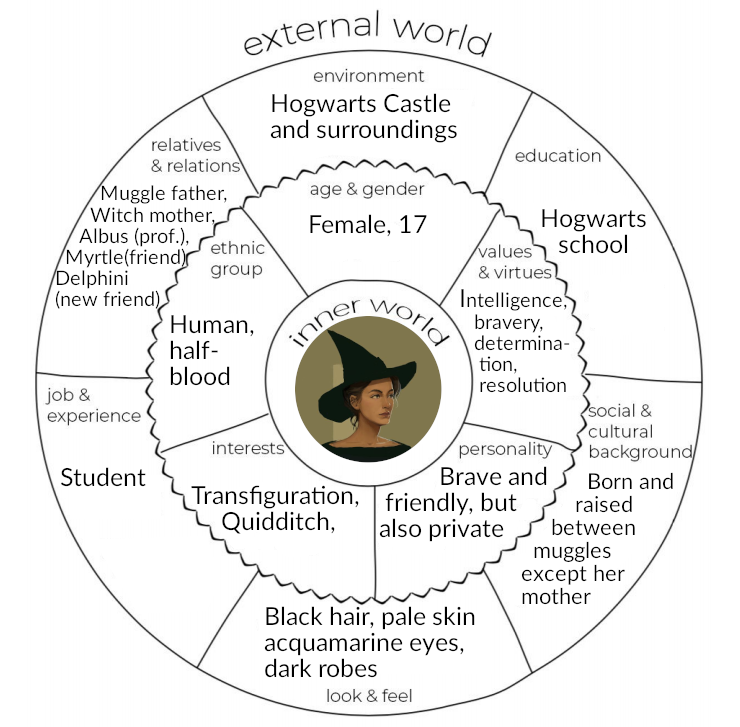
\includegraphics[max width=\textwidth]{../Pictures/Characters/Circumplexes/Minerva_circumplex.png} 
\captionsetup{labelformat=empty}
\caption{Circumplex}
\end{figure}

\begin{figure}[H]
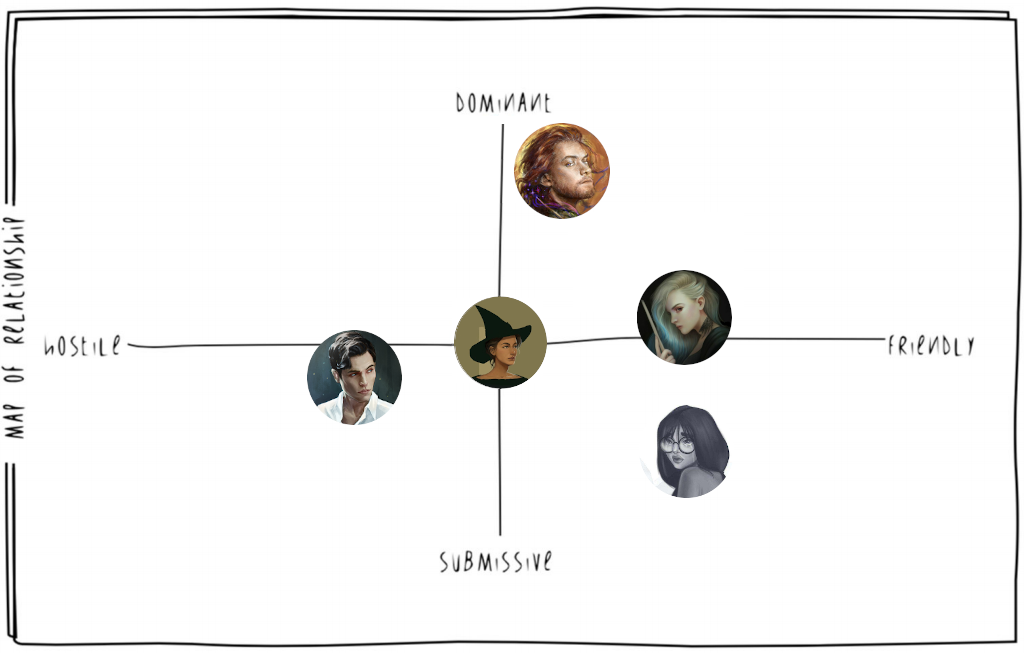
\includegraphics[max width=\textwidth]{../Pictures/Characters/Relationship_maps/Minerva_relmap.png} 
\captionsetup{labelformat=empty}
\caption{Map of relationships at the start of the game}
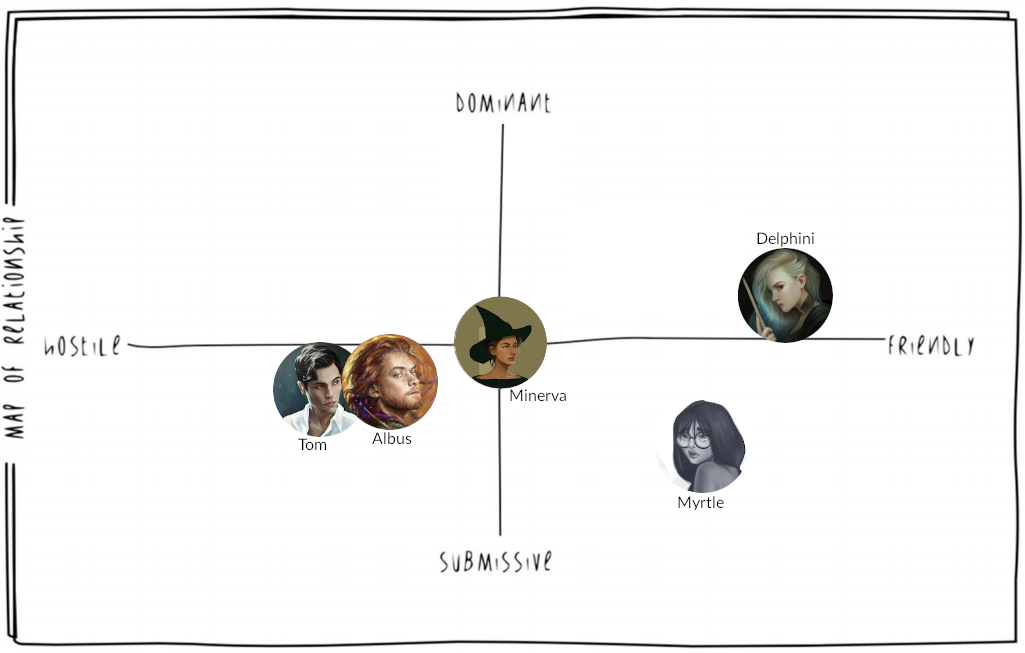
\includegraphics[max width=\textwidth]{../Pictures/Characters/Relationship_maps/Minerva_after_event_relmap.png} 
\captionsetup{labelformat=empty}
\caption{Map of relationships after the premature death of her dear friend Myrtle}
\end{figure}

\clearpage